\chapter{Evaluations and Results}
\markright{Aravindan Mahendiran \hfill Chapter 4. Evaluations and Results \hfill}
To evaluate our hypothesis about the vocabularies we test our models on eight different presidential elections from Latin America using both the seed vocabulary and the vocabulary generated by the query expansion algorithm.
We use the results obtained using the seed vocabulary detailed in the previous section as a baseline score.
We then use the same vocabulary to seed our PSL learning algorithm. 
The prediction algorithms are then run again, now by using the expanded vocabulary obtained through the query expansion.
In order to remain consistent with predicting ahead of time, we track only the hashtags identified by the query expansion pipeline  until that particular date.

\begin{figure*}
	\centering
	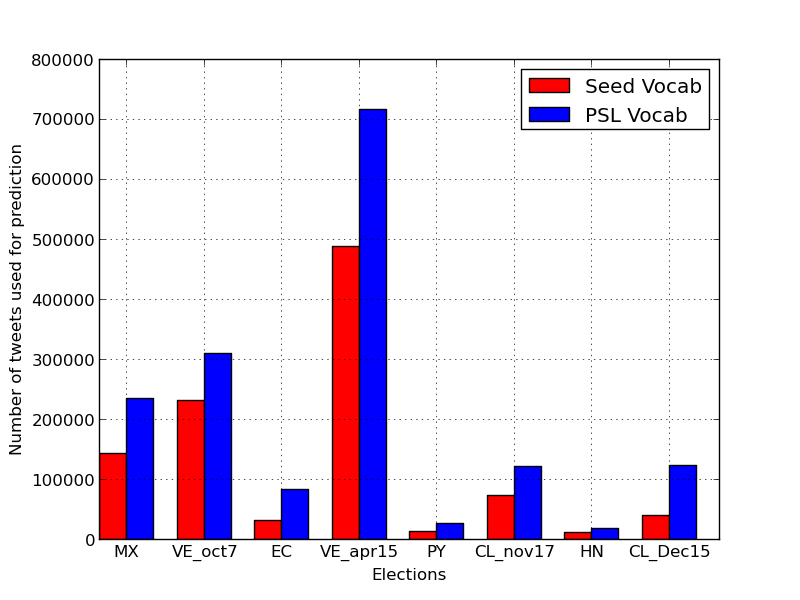
\includegraphics[scale=0.65]{support_files/Recall.png}
	\caption{Recall of seed vocabulary vs PSL vocabulary}
	\label{fig:recall}
\end{figure*}

Figure \ref{fig:recall} shows the increase in the number of documents that were used by the algorithms to make a predictions.
It is noticed when averaged across all the eight elections we notice close to a two-fold increase in the number of 
tweets that were used by these models.
This is a substantial increase of relevant tweets for the domain.

	\begin{table*}
		\centering
		\begin{tabular}{| l | l | r | r | r | r | r | r |}
		\hline
		Election & Candidate & Actual Result & Seed Vocab. & Error & PSL Vocab. & Error \\
		\hline
		\multirow{2}{*}{Mexico} & Pena Nieto & 38.1 & 49.26 & 11.11 & 46.43 & 8.28 \\\cline{2-7}
											   & Lopez Obrador & 31.64 & 25.11 & 6.53 & 27.65 & 4.00 \\
		\hline
		\multirow{2}{*}{Venezuela\_Oct7} & Hugo Chavez & 55.07 & 63.69 & 8.62 & 55.24 & 0.17\\\cline{2-7}
																& Henrique Capriles & 44.31 & 36.31 & 8.00 & 44.76 & 0.45 \\
		\hline
		\multirow{2}{*}{Ecuador} & Rafael Correa & 57.16 & 32.36 & 24.81 & 32.90 & 24.27 \\\cline{2-7}
												 & Guillermo Lasso & 22.68 & 36.93 & 14.25 & 37.88 & 15.20 \\
		\hline
		 \multirow{2}{*}{Venezuela\_Apr15} & Nicolas Maduro & 50.61 & 42.08 & 8.53 & 44.05 & 6.56 \\\cline{2-7}
																	& Henrique Capriles & 49.12 & 37.98 & 11.14 & 37.14 & 11.98 \\
		\hline
		\multirow{2}{*}{Paraguay} & Horacio Cartes & 48.48 & 29.80 & 18.68 & 29.12 & 19.36 \\\cline{2-7}
												   & Efrain Alegre & 39.05 & 27.21 & 11.84 & 26.63 & 12.42 \\
		\hline
		\multirow{2}{*}{Chile\_Nov17} & Michelle Bachelet & 46.70 & 26.62 & 20.08 & 29.92 & 16.78\\\cline{2-7}
														  & Evelyn Matthei & 25.03 & 18.76 & 6.27 & 19.52 & 5.51 \\
		\hline 
		\multirow{2}{*}{Honduras} & Orlando Hernandez & 36.80 & 28.94 & 7.86 & 34.74 & 2.06 \\\cline{2-7}
												   & Xiomara Castro & 28.70 & 9.67 & 19.03 & 14.20 & 14.50 \\
		\hline
		\multirow{2}{*}{Chile\_Dec15} & Michelle Bachelet & 62.16 & 57.66 & 4.50 & 59.24 & 2.92\\\cline{2-7}
															& Evelyn Matthei & 37.83 & 42.34 & 4.51 & 40.67 & 2.84 \\
		\hline 											 
		\end{tabular}
		\caption{Reduction in prediction error for Unique Visitor Model. All values shown are percentages.}
		\label{table:UniVis}
	\end{table*}


\begin{table*}
		\centering
		\begin{tabular}{| l | l | r | r | r | r | r | r |}
		\hline
		Election & Candidate & Actual Result & Seed Vocab. & Error & PSL Vocab. & Error \\
		\hline
		\multirow{2}{*}{Mexico} & Pena Nieto & 38.1 & 46.80 & 8.65 & 39.00 & 0.85 \\\cline{2-7}
											   & Lopez Obrador & 31.64 & 24.67 & 6.97 & 28.64 & 3.00 \\
		\hline
		\multirow{2}{*}{Venezuela\_Oct7} & Hugo Chavez & 55.07 & 49.89 & 5.18 & 55.89 & 0.82\\\cline{2-7}
																& Henrique Capriles & 44.31 & 36.31 & 8.00 & 43.91 & 0.40 \\
		\hline
		\multirow{2}{*}{Ecuador} & Rafael Correa & 57.16 & 53.33 & 3.84 & 54.33 & 2.84 \\\cline{2-7}
												 & Guillermo Lasso & 22.68 & 12.27 & 10.41 & 12.75 & 9.93 \\
		\hline
		 \multirow{2}{*}{Venezuela\_Apr15} & Nicolas Maduro & 50.61 & 51.45 & 0.84 & 50.58 & 0.03 \\\cline{2-7}
																	& Henrique Capriles & 49.12 & 35.96 & 13.16 & 38.11 & 11.01 \\
		\hline
		\multirow{2}{*}{Paraguay} & Horacio Cartes & 48.48 & 35.21 & 13.27 & 40.63 & 7.85 \\\cline{2-7}
												   & Efrain Alegre & 39.05 & 31.33	 & 7.72 & 34.44 & 4.62 \\
		\hline
		\multirow{2}{*}{Chile\_Nov17} & Michelle Bachelet & 46.70 & 38.91 & 7.79 & 41.80 & 4.91\\\cline{2-7}
														  & Evelyn Matthei & 25.03 & 19.20 & 5.83 & 20.98 & 4.05 \\
		\hline 
		\multirow{2}{*}{Honduras} & Orlando Hernandez & 36.80 & 25.16 & 11.64 & 28.30 & 8.50 \\\cline{2-7}
												   & Xiomara Castro & 28.70 & 16.53 & 12.17 & 24.90 & 3.80 \\
		\hline
		\multirow{2}{*}{Chile\_Dec15} & Michelle Bachelet & 62.16 & 39.12 & 23.04 & 39.80 & 22.37\\\cline{2-7}
															& Evelyn Matthei & 37.83 & 20.88 & 16.95 & 21.68 & 16.15 \\
		\hline 											 
		\end{tabular}
		\caption{Reduction in prediction error for Regression Model. All values shown are percentages.}
		\label{table:RegModel}
	\end{table*}
	
To further illustrate the fact that the vocabulary used by such algorithms plays a vital role, we compare the performance of the models using the two different vocabularies.
To reduce the effect of outliers we track the popularity of only the top two candidates from each election.
Table~\ref{table:UniVis} shows the reduction in prediction error for the Unique Visitor model for each candidate if the expanded vocabulary from the PSL approach is used instead of the seed vocabulary.
On an average the error was reduced by a 28.60\% from the original prediction error obtained by using seed vocabulary.
Similarly Table~\ref{table:RegModel} shows the reduction in error for the Regression Model.
Here an even better improvement of 45.19\% reduction in error was noted.
Averaging the reduction in error for both the models, the query expansion exercise was able to reduce the prediction error by  36.90\%.
We see greater and more consistent improvement with the regression model as the model weighs each window of tweets differently depending upon the opinion poll time series whereas the unique visitor model values them equally. 
Therefore, when the algorithm uses the `not-so-informative' hashtags identified during 
the earlier iterations, the sentiment value and the counts of these mentions bring down the accuracy of the model even though at a later stage hash-tags that are strongly indicative of a user's preference is picked up.
So words such as "facebook" which occur commonly dominate the counts and therefore skew the results even though they are dropped from the vocabulary at a later point.